%\setcounter{page}{1}
\setcounter{equation}{0}
\setcounter{figure}{0}

\section{A Theory for the $\rm CO_2$ Molecule}

Name \rule{2.0in}{0.1pt}\hfill{}Section \rule{1.0in}{0.1pt}\hfill{}Date
\rule{1.0in}{0.1pt}

\textbf{Objective}

To use a numerical technique to solve the Schroedinger equation for the harmonic oscillator,
compare calculations with measurements from $\rm CO_2$,
 and explore
the implications of the quantum theory especially the quantization of energy
in bound systems.

\textbf{Apparatus}

\begin{itemize}

\item {\it Schr\"odinger Shooter} software

\end{itemize}

\textbf{Overview}

Quantum mechanics is the theoretical structure used to make sense of the atomic and sub-atomic
world. 
It is based on a small set of assumptions and a lot of associated mathematics.

\begin{center}
\bf The Postulates of Quantum Mechanics
\end{center}

\begin{enumerate}

\item The quantum state of a particle is characterized by a wave function  
$\Psi(\vec r,t)$, which contains all the information about the system an observer can 
possibly obtain.
The square of the magnitude of the wave function $|\Psi (\vec r,t)|^2$ 
is interpreted as a probability or probability density for the particle's presence. 

\item The things we measure ({\it e.g.} energy, momentum) are called observables. 
Each observable has a corresponding mathematical object called an operator 
that does `something' to the wave function $\Psi(\vec r,t)$ to generate the value of the observable.
The spatial dependence of the wave function in one dimension $\Psi(x,t)$ is governed by
the energy operator which generates a famous expression called the
Schr\"odinger equation
\begin{equation}
-\frac{\hbar^2}{2 m}\frac{d^2}{d x^2} \psi(x) + V \psi(x) = E  \psi(x)
\end{equation}
where $\hbar$ is Planck's constant, $m$ is the mass of the particle, and $V$ is the potential
energy of the particle.
Ultimately, the success of this approach will depend on how the theoretical
results we generate from solving the Schr\"odinger equation compare with
measurements.

\end{enumerate}

\noindent We will focus on these postulates in this laboratory and in particular
on understanding and solving Equation 1, the Schr\"odinger equation.

\textbf{Activity 1: The Harmonic Oscillator Energy in One  Dimension}


Consider the form of the total
mechanical energy of a particle in one dimension
\begin{equation}
E =    \frac{1}{2} m v^2 + V(x) 
\end{equation}
where $m$ is the particle's mass, $v$ is its
velocity, and  $V(x)$ is the potential energy of the particle
and depends only on the particle's position.
The potential energy of a particle undergoing simple harmonic motion is
\begin{equation}
V(x) = \frac{kx^2}{2}
\end{equation}
where we have set the origin at the equilibrium point of the harmonic oscillator.

\newpage

(a) Make a sketch of the potential energy as a function of $x$.
What are the limiting values of the potential?
\vskip 3.5cm

(b) Since the energy is constant you can draw it on your previous sketch as a flat, straight
line. We are considering bound states.
Draw an energy line for a bound state on your previous sketch.
Does your energy `curve' intersect the effective potential curve anywhere?
For a classical particle like a ball rolling on a hill or a satellite orbiting the
Earth,
what happens at this intersection?
Describe the motion of a classical particle in this potential.
What restrictions are there on the energy $E$ of a classical particle?
\vskip 3.0cm

\textbf{Activity 2: Quantum Predictions}

(a) What do you expect the square of the wave function of the harmonic oscillator to look like?
Copy your drawing from part 1.a and add
a sketch of your expectation for the harmonic oscillator probability density on the same graph. 
\vskip 5.0cm

(b) What happens to the square of your wave function as the energy increases?
Make another copy here of the graph of the effective potential energy that you made in 2.a.
Draw an energy curve for a higher energy state than your previous one.
Now sketch the new, higher-energy wave function.
How is it different from the curve you made in 2.a?
\vskip 5.0cm

\newpage

\textbf{Activity 3: Solving the Schr\"odinger Equation}

(a) We are now ready to start solving the Schr\"odinger Equation.
Go first to the {\tt All Programs} menu, then
to {\tt Physics Applications} and click on {\tt Schr\"odinger Shooter}.
You will see the {\tt Schr\"odinger Shooter} window like the one in the next figure.
If you don't see this window, consult your instructor.
\begin{figure}[hbt]
\begin{center}
\includegraphics[width=6.0in]{solveSE/shooter1b.eps}
\caption{Initial panel for {\it Schr\"odinger Shooter}}
\end{center}
\end{figure}

(b) The first step is to select a potential energy function.
Click on {\tt File} and go to {\tt New Potential Energy Function}.
Select the potential energy function for the harmonic oscillator.
Set the spring constant to $k=2.4$ by clicking in the box labeled {\tt K:}
and entering the value.
Use the second menu button from the left-hand side 
at the bottom of the {\tt Schr\"odinger Shooter}
window to choose {\tt Normalized} wave functions (it should be labeled {\tt Not Normalized}
when you start the program).
This last choice makes it easier to compare wave functions for different quantum numbers.
Last, set the initial value of the energy to 0.1 in the box labeled 
{\tt Energy (Rydbergs):} and hit return.
The conversion between eV and rydbergs is normally $\rm 13.605 6923(12)~ eV/rydberg$,
but we rescale that value here so it is $\rm 0.13605 6923(12)~ eV/rydberg$.
The number in parentheses is the uncertainty on the last two digits in the
experimental value.
At this point you should see curves in both of the panels of the 
{\tt Schr\"odinger Shooter} window.
If you don't, consult your instructor.

\newpage

(c) You should see several curves in the upper panel.
What quantities do the light blue, red, yellow, and green curves represent?
Use the legend in the lower right portion of the {\tt Schr\"odinger Shooter}
window.
Record them here.
\vspace{2.5cm}

(d) You can now adjust the energy of the particle in the harmonic oscillator potential to find 
the energy levels.
There are three ways to change this energy.
There is a slide on the left-hand side of the {\tt Schr\"odinger Shooter} window.
Click and drag the slide to change the energy and read the value
in the box labeled {\tt Energy(Rydbergs)} located near the top of the 
{\tt Schr\"odinger Shooter} window.
You can also enter the energy in the same box
labeled {\tt Energy(Rydbergs):} as you did in part 3.b.
Last, to the right of this last box there are buttons labeled
{\tt Adjust Energy:} that will increase or decrease the energy and change the step size.

(e) Tune the energy to find lowest four energy levels in your harmonic oscillator by obtaining
physically acceptable wave functions.
You may need to increase the horizontal range to view the full wave function.
You can do this by increasing the value in the box labeled {\tt Cutoff:} at the
bottom of the {\tt Schr\"odinger Shooter} window.
If you increase the horizontal scale, then increase the next box labeled
{\tt Count:} (next to the {\tt Cutoff} box) by the same ratio.
In other words, if you double the cutoff, then double the count.
This last parameter controls the stepsize used in the numerical integration of
the Schr\"odinger equation.
What does the wave function look like when you have found the correct energy level?
What postulate did you exploit to find the correct solutions?
How does the radial wave function change as the energy increases?
Record you values for each of the energy levels below.

\vspace{9.0cm}

\textbf{Activity 4: Analysis and Comparison with Data}

(a) Enter the values you found for the energies in an {\it Excel} spreadsheet
and convert the values to eV.
Use the scale below to make an energy level diagram for your harmonic oscillator calculations.

\newpage

\vspace{0.25in}

\hspace{1.0cm}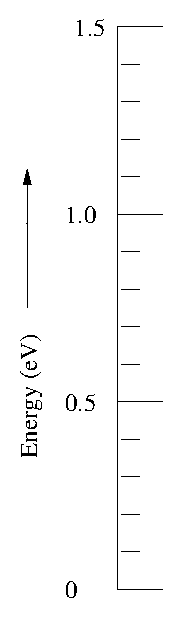
\includegraphics{solveSE/energyLevels2.eps}

\vspace{0.5in}

(b) When molecules absorb energy they `jump' to higher energy quantum states.
When they `cool off' they emit radiation as they go down in energy from one state to 
the next. For the energy level diagram you drew in the previous Activity what is the difference 
in energy $\Delta E$ between the successive levels? What is the relationship between
the ground state energy and $\Delta E$?

\vspace{4.0cm}

\newpage

(c) The plot below shows the absorption spectrum of $\rm CO_2$ as a function of wavenumber $k$.
From the plot read off the peak $k$ values of the different absorption lines and convert them to energies 
with $E_\gamma = hck$ where $h$ is Planck's constant and $c$ is the speed of light.
Use the widths of the peaks as the uncertainty.

\includegraphics[width=4.0in]{solveSE/CO2absorption1.eps}

\vspace{1.5cm}

(c) Compare your calculated results with the measurements of the transitions observed in $\rm CO_2$. 
What is the difference between the two sets in terms of the uncertainty on the measurement?
\vspace{2.5cm}


\textbf{Activity 5: The Meaning of Quantum Theory}

(a)  Return to the questions in Activity 2 and examine your predictions.
How did you do?
Correct any statements that you now find are wrong.
\vspace{2.0cm}

(b) What requirement or postulate forces us to choose particular energy states
({\it i.e.} what causes energy quantization)?
\vspace{2.0cm}


(c) Consider a variation of one of the questions in part 1.b.
In that question you were asked to describe the motion of a classical particle
like a satellite orbiting the Earth.
Describe the motion of a quantum particle in the harmonic oscillator potential.
\vspace{3.0cm}

\newpage

\textbf{Homework}

\begin{enumerate}

\item An atom absorbs a photon whose frequency is
$f = 6.2\times 10^{14}~Hz$.
How much does the energy of the atom increase?

\item The value of $\omega$ for the carbon monoxide molecule $\rm CO$ is $4.03\times 10^{14}~rad/s$.
What are the energy and wavelength of a photon emitted when the $\rm CO_2$
harmonic oscillator
undergoes a transition from the $n=3$ state to the $n=2$ state?

\item The relationship between the spring constant $k$ and the characteristic angular frequency $\omega$
is $k = \mu \omega^2$ where $\mu$ is the reduced mass. 
For a diatomic atom we characterize the mass of oscillator with this reduced mass 
$\mu = m_1 m_2/(m_1+m_2)$ where $m_1$ and $m_2$ are the masses of the atoms in the 
molecule.
Use the data for $\rm CO$ in the previous problem to determine the spring constant
for the $\rm CO$ molecule.

\item The $\rm HCl$ molecule shows a strong absorption line at the frequency $f=8.66\times 10^{13} ~Hz$.
What is the effective spring constant $k$ for $\rm HCl$? 
What is the classical amplitude of vibration
for a $\rm HCl$ molecule in the $n=0$ vibrational state?
Compare your result for the spring constant with the value of $k$ for our typical lab springs which
are in the range $k=10-30~N/m$.

\item Draw Lewis structures for the $\rm HCl$ and $\rm CO$ molecules discussed above. Compare the 
spring constants you calculated for the molecules and their Lewis structures.
What conclusions can you draw, if any, about the relationship between the spring constants
and the molecular bonds?


\end{enumerate}
